%% To submit your paper:
\documentclass[draft]{agujournal2019}
\usepackage{url} %this package should fix any errors with URLs in refs.
\usepackage{lineno}
\usepackage[inline]{trackchanges} %for better track changes. finalnew option will compile document with changes incorporated.
\usepackage{soul}
\linenumbers
%%%%%%%
% As of 2018 we recommend use of the TrackChanges package to mark revisions.
% The trackchanges package adds five new LaTeX commands:
%
%  \note[editor]{The note}
%  \annote[editor]{Text to annotate}{The note}
%  \add[editor]{Text to add}
%  \remove[editor]{Text to remove}
%  \change[editor]{Text to remove}{Text to add}
%
% complete documentation is here: http://trackchanges.sourceforge.net/
%%%%%%%

\draftfalse

\journalname{Geophysical Research Letters}


\begin{document}

%% ------------------------------------------------------------------------ %%
%  Title
%
% (A title should be specific, informative, and brief. Use
% abbreviations only if they are defined in the abstract. Titles that
% start with general keywords then specific terms are optimized in
% searches)
%
%% ------------------------------------------------------------------------ %%



\title{Duration of Individual Relativistic Electron Microbursts: A Probe Into Their Scattering Mechanism}

\authors{M. Shumko\affil{1, 2}, L.W. Blum\affil{3}, and A.B. Crew\affil{4}}

\affiliation{1}{NASA's Goddard Space Flight Center, Greenbelt, Maryland, USA}
\affiliation{3}{Universities Space Research Association, Columbia, Maryland, USA}
\affiliation{3}{University of Colorado Boulder, Boulder, Colorado, USA}
\affiliation{2}{Johns Hopkins University Applied Physics Laboratory, Laurel, Maryland, USA}

\correspondingauthor{M. Shumko}{msshumko@gmail.com}

%% Keypoints, final entry on title page.

%  List up to three key points (at least one is required)
%  Key Points summarize the main points and conclusions of the article
%  Each must be 100 characters or less with no special characters or punctuation and must be complete sentences

\begin{keypoints}
\item We identified relativistic microbursts observed by the SAMPEX satellite and quantified their duration
\item The microburst duration is shortest at midnight and longest at noon magnetic local times
\item Whistler-mode chorus rising tone element duration has a similar trend \textcolor{red}{Update?}
\end{keypoints}

%% ------------------------------------------------------------------------ %%
%
%  ABSTRACT and PLAIN LANGUAGE SUMMARY
%
% A good Abstract will begin with a short description of the problem
% being addressed, briefly describe the new data or analyses, then
% briefly states the main conclusion(s) and how they are supported and
% uncertainties.

% The Plain Language Summary should be written for a broad audience,
% including journalists and the science-interested public, that will not have 
% a background in your field.
%
% A Plain Language Summary is required in GRL, JGR: Planets, JGR: Biogeosciences,
% JGR: Oceans, G-Cubed, Reviews of Geophysics, and JAMES.
% see http://sharingscience.agu.org/creating-plain-language-summary/)
%
%% ------------------------------------------------------------------------ %%

%% \begin{abstract} starts the second page

\begin{abstract}
In this study we used the Solar Anomalous and Magnetospheric Particle Explorer to identify relativistic, $>1$ MeV, electron microbursts and we quantified their duration. We found the shortest microbursts, with a median duration around 80 milliseconds, near midnight magnetic local time. Microburst duration increases through dawn and to noon magnetic local time, where the median microburst duration roughly doubles to 160 milliseconds. The increasing microburst duration trend in magnetic local time is similar to the whistler mode chorus rising tone element duration, shedding light into the microburst scattering mechanism.
\end{abstract}

\section*{Plain Language Summary}
\noindent Microbursts are a naturally occurring form of electron precipitation from the near-Earth space into the atmosphere. They are characterized by their short duration, typically defined to be less than a second, or sometimes as 100 milliseconds... Microburst impact on the atmosphere includes the degradation of Mesospheric Ozone through the production of Odd Nitrogen and Odd Hydrogen molecules... We don't know the details on how microburst electrons are scattered, but there is evidence that they are scattered by whistler-mode chorus rising tone elements... Talk about duration and how it is a probe into the scattering physics.

\section{Introduction}\label{intro}
Earth's outer radiation belt particle population is in constant flux, governed by many processes that affect particles via, for example: radial transport with injections from the magnetotail and ultra low frequency waves, local heating and loss into Earth's atmosphere due to wave-particle interactions \textcolor{red}{Cite Ripoll et al., 2019 "Particle Dynamics in the Earth's Radiation Belts: Review of Current Research and Open Questions"}. Whistler mode chorus (WMC) is just one type of plasma wave characterized by short ($\approx 100$ ms) rising tone elements, and perform a dual role in electron dynamics: accelerating electrons from $\approx 10$ keV injection energies up to MeV energies, and pitch angle scattering electrons into the atmosphere \cite<e.g.>{Li2009b, Thorne2010, Horne2003a, Summers2005}. One form of electron precipitation is microbursts: a transient and intense increase of electrons, with a $\approx 100$ ms duration, first observed by balloons in Earth's upper atmosphere, and later by satellites in low Earth orbit (LEO), and recently at high altitude near the magnetic equator \cite<e.g.>{Anderson1964, Blake1996, Lorentzen2001a, O'Brien2003,Douma2017, Kurita2016, Shumko2018b}.

Microburst electron energies span multiple orders of magnitude from tens of keV observed by, for example, \citeA{Datta1997}; to $>1$ MeV observed by the Solar Anomalous Magnetospheric Particle Explorer (SAMPEX) by \citeA{Blum2015}. Microbursts are predominately observed outside the plasmapause on the radiation belt footprints, $L\approx4-8$, and in the midnight to morning Magnetic Local Times (MLT) ($\approx 0-12$ hours MLT) \cite{Lorentzen2001a, Blum2015, O'Brien2003, Douma2017}. While microbursts are observed under all geomagnetic conditions, \citeA{Douma2017} showed that microburst frequency dramatically increases with the Auroral Electrojet (AE) index, and \citeA{O'Brien2003} showed a similar trend with the microburst frequency with the Disturbance storm time index.

The relative impact of microbursts on the ionization of Earth's atmosphere and the depletion of radiation belt electrons is uncertain \textcolor{red}{cite something}, but the impact of microbursts alone is estimated to be substantial. Microbursts can deplete the outer radiation belt electrons in as little as a few hours, and can deplete up to 20\% of upper mesospheric ozone \cite{O'Brien2004, Thorne2005, Douma2019,Breneman2017,Seppala2018}.

Electron microbursts are believed to be scattered by chorus waves. They were associated early on, due to the similar duration of microbursts and chorus rising tone elements, and a similar occurrence distributions in MLT \cite<e.g.>{Lorentzen2001a}. \citeA{Breneman2017} directly linked a chorus rising tone element to a microburst observed by the Focused Investigation of Relativistic Electron Bursts: Intensity, Range, and Dynamics CubeSats (FIREBIRD-II; \citeA{Johnson2020}) during a close magnetic conjunction. With this evidence, the particle precipitation community is largely in agreement that chorus waves scatter microbursts. 

A natural follow-on question is how. For example, it is still unclear if relativistic ($>1$ MeV) microbursts are scattered via cyclotron resonance at high magnetic latitudes, or a higher resonance harmonic near the magnetic equator \cite{Lorentzen2001a}. One way to address this question is by studying for how long microburst electrons are in resonance with a chorus wave. The resulting microburst duration, i.e. the microburst peak width in the time series data, is a probe into the conditions necessary to scatter microburst electrons. From our literature review, we found only qualitative estimates of the microburst duration. Therefore, we used the microbursts observed by the SAMPEX satellite to quantify the distribution of $>1$ MeV microburst duration. In this letter, we quantify the duration distribution of microbursts as a function of L-shell, MLT, and the Auroral Electrojet. We then compare these results to prior chorus rising tone element studies, and a chorus-electron scattering model. 

\section{Instrumentation}\label{instrumentation}
In this study we used the $>1$ MeV electron count data, taken by the Heavy Ion Large Telescope (HILT) instrument \cite{Klecker1993}, that was onboard the SAMPEX satellite \cite{Baker1993}.

SAMPEX was launched in July 1992 and reentered Earth's atmosphere in November 2012. It was in a 520x670 km, $82^\circ$ inclination low Earth orbit. In general, the SAMPEX had two pointing modes: spin and orbit rate rotation (zenith pointing) modes. To avoid the compounding effects due to the variable pitch angles sampled in the spin mode, we only used the zenith pointing mode data. The International Geomagnetic Reference Field \cite[IGRF]{Thebault2015} magnetic field model was used to derive the meomagnetic coordinates.

We used the HILT electron data, sampled at a 20 ms cadence (state4 in the data archive), that was taken between 1997 and 2012. The HILT instrument consisted of a large rectangular chamber with the aperture on one end, and 16 solid state detectors on the other. The electron counts accumulated over 20 ms were summed from all of the solid state detectors and used in this study.

The HILT instrument is ideal for studying relativistic microbursts and it was used in many prior microburst studies including \citeA{O'Brien2003, Lorentzen2001a, Blake1996, Nakamura2000, Kurita2016}, and \citeA{Douma2017}.

\section{Methodology}\label{methodology}

To estimate the microburst duration we first identified microbursts and then we fit them with a Gaussian model with a linear trend to quantify the duration for each microburst.

\subsection{Microburst Identification}\label{microburst_id}
We identified microbursts using the burst parameter defined by \citeA{O'Brien2003} and used in numerous other microburst studies with SAMPEX \cite<e.g.>{Douma2017}. Assuming Poisson probability for the observed electron counts, the burst parameter is the number of standard deviations of a foreground signal above the background, expressed as
\begin{equation}
n_\sigma = \frac{N-A}{\sqrt{A+1}}
\end{equation} where $N$ is the number of foreground electron counts (microburst or otherwise), and $A$ is the centered running average background counts. The $1$ in the denominator prevents a division by 0 error. In \citeA{O'Brien2003}, and in the results in this study, $N$ was summed over 0.1 seconds and is called $N_{100}$, while $A$ was summed over 0.5 seconds and is called $A_{500}$.  Henceforth we will specify the time window with the subscript for $N$ and $A$. Times when $n_\sigma > 10$ are classified as microburst times, and the peak count rate in each time interval is saved as a microburst to our data set. With $A_{500}$ and $N_{100}$, we detected a total of 256,764 microbursts over the 15 year period from 1997 to 2012. Four examples of microbursts are shown in Fig. \ref{fig1} by the solid black curves.

\textcolor{blue}{Check the argument for clarity} The choice of $A$ determines the sensitivity of the burst parameter to microbursts of various durations (widths). This sensitivity is best illustrated with an example. Given a 1-second wide microburst, if we use $A_{500}$, the centered average background at the microburst time is skewed towards the microburst peak and the microburst's $\mathrm{bp}$ is reduced, potentially below the detection threshold. On the other hand, if we use $A_{1000}$, the centered running background will be relatively less elevated at the microburst time so it has a greater $\mathrm{bp}$ and is more likely to be detected. In other words, $bp$ will be relatively larger for $A_{1000}$ than $A_{500}$. This sensitivity manifests itself as a bias towards detecting narrower microbursts that we will address later in this study. 

\begin{figure}
\noindent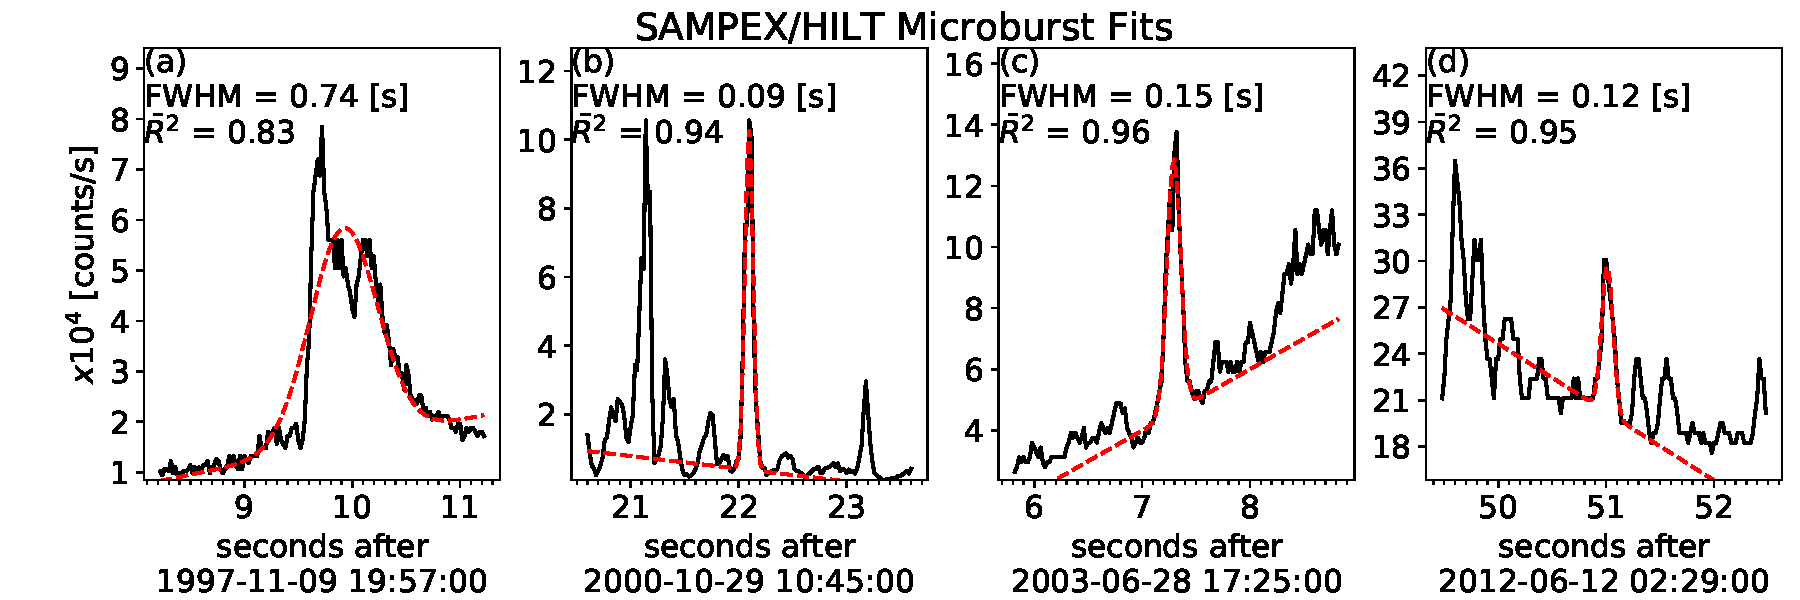
\includegraphics[width=\textwidth]{figures/fig1.pdf}
\caption{Examples $>1$ MeV microbursts are shown by the black lines, and the fits are shown by the dashed red lines. The fit full width at half maximum (FWHM) and the $\bar{R}^2$ goodness of fit metric is annotated in each panel. Microbursts with $\bar{R}^2 > 0.9$ were used for this study. The major time ticks are at every second, while the minor ticks are at every 100 milliseconds.}
\label{fig1}
\end{figure}

\subsection{Microburst Duration}
We estimated the microburst duration using two methods that yielded similar results: the duration at half of the microburst's topographic prominence and duration from a Gaussian fit.

The topographic prominence is a simple and robust method to estimate the microburst duration used to identify curtains a similar-looking type of precipitation \cite{Shumko2020b}. It is defined as the duration at half of the microburst topographic prominence: the height of the microburst relative to the maximum of the two minima on either side of the microburst peak. On each side of the microburst peak, the minima are searched for between the microburst and a higher peak on that side. While the topographic prominence method of estimating microburst durations is simple and robust, one of its downsides is its inability to automatically verify that the duration is representative of a single microburst. Therefore, we also fit microbursts with a Gaussian, and used the $R^2$ goodness of fit metric to filter out bad duration estimates.

The other method that we use to estimate the microburst duration is fitting a Gaussian shape to microbursts. The advantage of this method is that it allows us to evaluate the fit using a goodness of fit metric. By screening out bad fits, we exclude superposition of multiple microbursts that will unintentionally bias our microburst duration estimate.

We assumed a Gaussian superposed with a linear trend fit model. The Gaussian models the shape of the microburst; while the linear trend accounts for the electrons that are either trapped or quasi-trapped in the drift loss cone. The fit model is defined as:
\begin{equation}
c(t | A, t_0, \sigma, c_0, c_1) = A e^{-\frac{(t-t_0)^2}{2\sigma^2}} + c_0 + c_1 t
\end{equation} where $A$, $t_0$, and $\sigma$ are the Gaussian amplitude, center time, and standard deviation; while the $c_0$ and $c_1$ are the background count intercept and slope. The fit was applied over a number of data points determined by the maximum of either: 4x topographic prominence width or 0.5 seconds. A challenge to any robust and automated nonlinear regression algorithm is guessing the initial parameters. The initial parameter guesses for the Gaussian are provided by the topographic prominence and topographic duration estimates. The two linear trend initial parameters were: $c_0=\mathrm{median(counts)}$ and $c_1=0$. The optimal fit parameters were found using scipy's \url{curve_fit()} function in Python. We defined the microburst duration as the full width at half maximum (FWHM) of the microburst peak, defined as
\begin{equation}
\mathrm{FWHM} = 2\sqrt{2 \ln{2}} \sigma.
\end{equation}

To evaluate the fit, we used the $R^2$ goodness of fit metric. $R^2$ is defined as
\begin{equation}
R^2 = 1 - \frac{SS_{res}}{SS_{mean}} = 1 - \frac{\sum{(c_i-f_i)^2}}{\sum{(c_i-\bar{c})^2}}
\end{equation} where $SS_{res}$ is the sum of the squared residuals between the observed counts $c_i$ and the fit counts $f_i$ for each time step, and likewise $SS_{mean}$ is the sum of the squared residuals between $c_i$ and the mean of the counts, $\bar{c}$.

One interpretation of $R^2$ is: fractionally how much better is the variance in the data explained by the model fit, compared to the null hypothesis horizontal line at $\bar{c}$. $R^2$ values vary from $1$ when the fit perfectly describes the variance in the data, to $-\infty$ for poor fits (a fit can be much worse than the mean null hypothesis).

To account for overfitting that results from the variable number of data points used for each fit, the adjusted $R^2$, $\bar{R}^2$, was used. It is defined as

\begin{equation}
\bar{R}^2 = 1 - (1-R^2) \frac{n-1}{n-p-1}
\end{equation} where $n$ is the number of data points fit, and $p$ is the number of parameters. Intuitively, $n-1$ is the number of degrees of freedom for the null hypothesis, and $n-p-1$ is the degrees of freedom for the fit model. Fits with $\bar{R}^2 > 0.9$ are considered good fits and are used for the rest of this analysis. We compared the microburst duration estimated with the prominence and fit methods. With the $\bar{R}^2 > 0.9$ constraint, we found that for $85\%$ of microbursts, the duration estimated by both methods agreed to within $25\%$.

Figure \ref{fig1}a shows an example of two superposed microbursts that had a fit $\bar{R}^2 = 0.83$ that were excluded from this study. On other hand, Fig. \ref{fig1}b-d show microbursts that were included in this study because the fit $\bar{R}^2 > 0.9$.

Lastly, Fig. \ref{fig1}c,d demonstrate the necessity of the linear fit to account for the changing background. The linear fit accounts for the non-zero mean background counts and the different amplitudes of the edges of the Gaussian. Of the 256,764 detected microbursts, 109,231 had $R^2 > 0.9$ and are used for the remainder of this study.

\section{Results}\label{results}
We used the well-fit microbursts to quantify the distribution of microburst duration (FWHM) for all microbursts, as a function of the Auroral Electroject, and as a function of L and MLT. We begin with the overall microburst distribution.

Figure \ref{fig2}a shows the distribution of all well-fit microbursts. This distribution is peaked with the median at 98 ms and quickly drops off. The interquartile range spans about a factor of two in microburst duration, from 67 to 140 ms. 

We then investigated the dependence of microburst duration as a function of geomagnetic activity. To be consistent with the prior wave and microburst studies, we use the AE index to quantify the level of geomagnetic disturbance. We adopt the same three AE intensity levels used in prior studies, such as \citeA{Li2009a}, \citeA{Douma2017}, and \citeA{Meredith2020}: $\mathrm{AE} < 100$, $100 < \mathrm{AE} < 300$, and $\mathrm{AE} > 300$, in units of nanotesla. Figure \ref{fig2}b shows the distribution of microburst duration as a function of AE. This distribution is qualitatively similar: gradually narrowing and shifting to shorter durations with increasing AE. The median microburst duration decreases from 129 ms for $0 < \mathrm{AE} < 100$ to 94 ms for $ \mathrm{AE} > 300$.

\begin{figure}
\noindent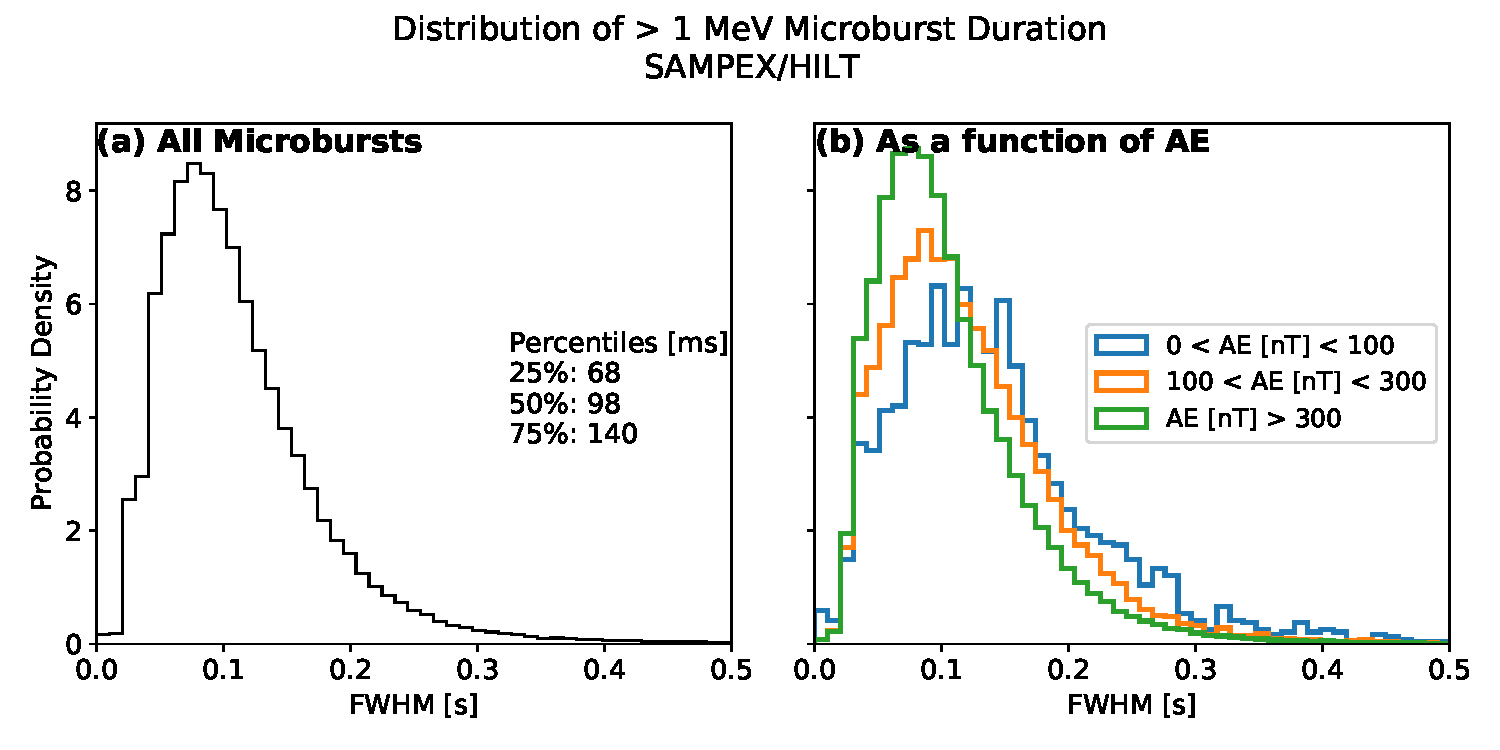
\includegraphics[width=\textwidth]{figures/fig2.pdf}
\caption{Panel a shows the distribution of all microburst full width at full maximum (FWHM). Panel b shows the distribution of all microbursts, categorized by the Auroral Electroject (AE) index into three bins: $0 < \mathrm{AE} < 100$, $100 < \mathrm{AE} < 300$, and $\mathrm{AE} > 300$, in units of nanotesla. The median microburst duration is 129 ms for the $0 < \mathrm{AE} < 100$, 110 ms for the $300 < \mathrm{AE} < 300$, and 94 ms for the $ \mathrm{AE} > 300$ categories.}
\label{fig2}
\end{figure}

Lastly, we investigated the duration distribution as a function of L and MLT. The joint distribution is shown in Fig. \ref{fig3}. Figure \ref{fig3}a-c show the 25\%, 50\%, and 75\% percentiles of microburst durations in each L-MLT bin. The sparse bins with less than 100 well-fit microbursts are white. For reference, Fig. \ref{fig3}d shows the number of well-fit microbursts observed as a function of L and MLT.

Figure \ref{fig3} shows that the microburst duration trend is almost identical for the different percentiles, so for simplicity we focus on the median distribution in Fig. \ref{fig3}b. In MLT, the median microburst duration increases by a factor of two: from 80 ms at midnight to 160 ms at noon. In L-shell, the median microburst duration slightly increases with L shell, most apparent near midnight MLT. To disentangle the L and MLT distribution, Fig. \ref{fig4} shows the marginalized distributions; MLT was marginalized out in Fig. \ref{fig4}a and L-shell was marginalized out in Fig. \ref{fig4}b. Figure \ref{fig4}a shows a slight broadening of the microburst duration at higher L-shells; in contrast to Fig. \ref{fig4}b that clearly shows that the microburst duration increases from midnight to noon MLT.

\begin{figure}
\noindent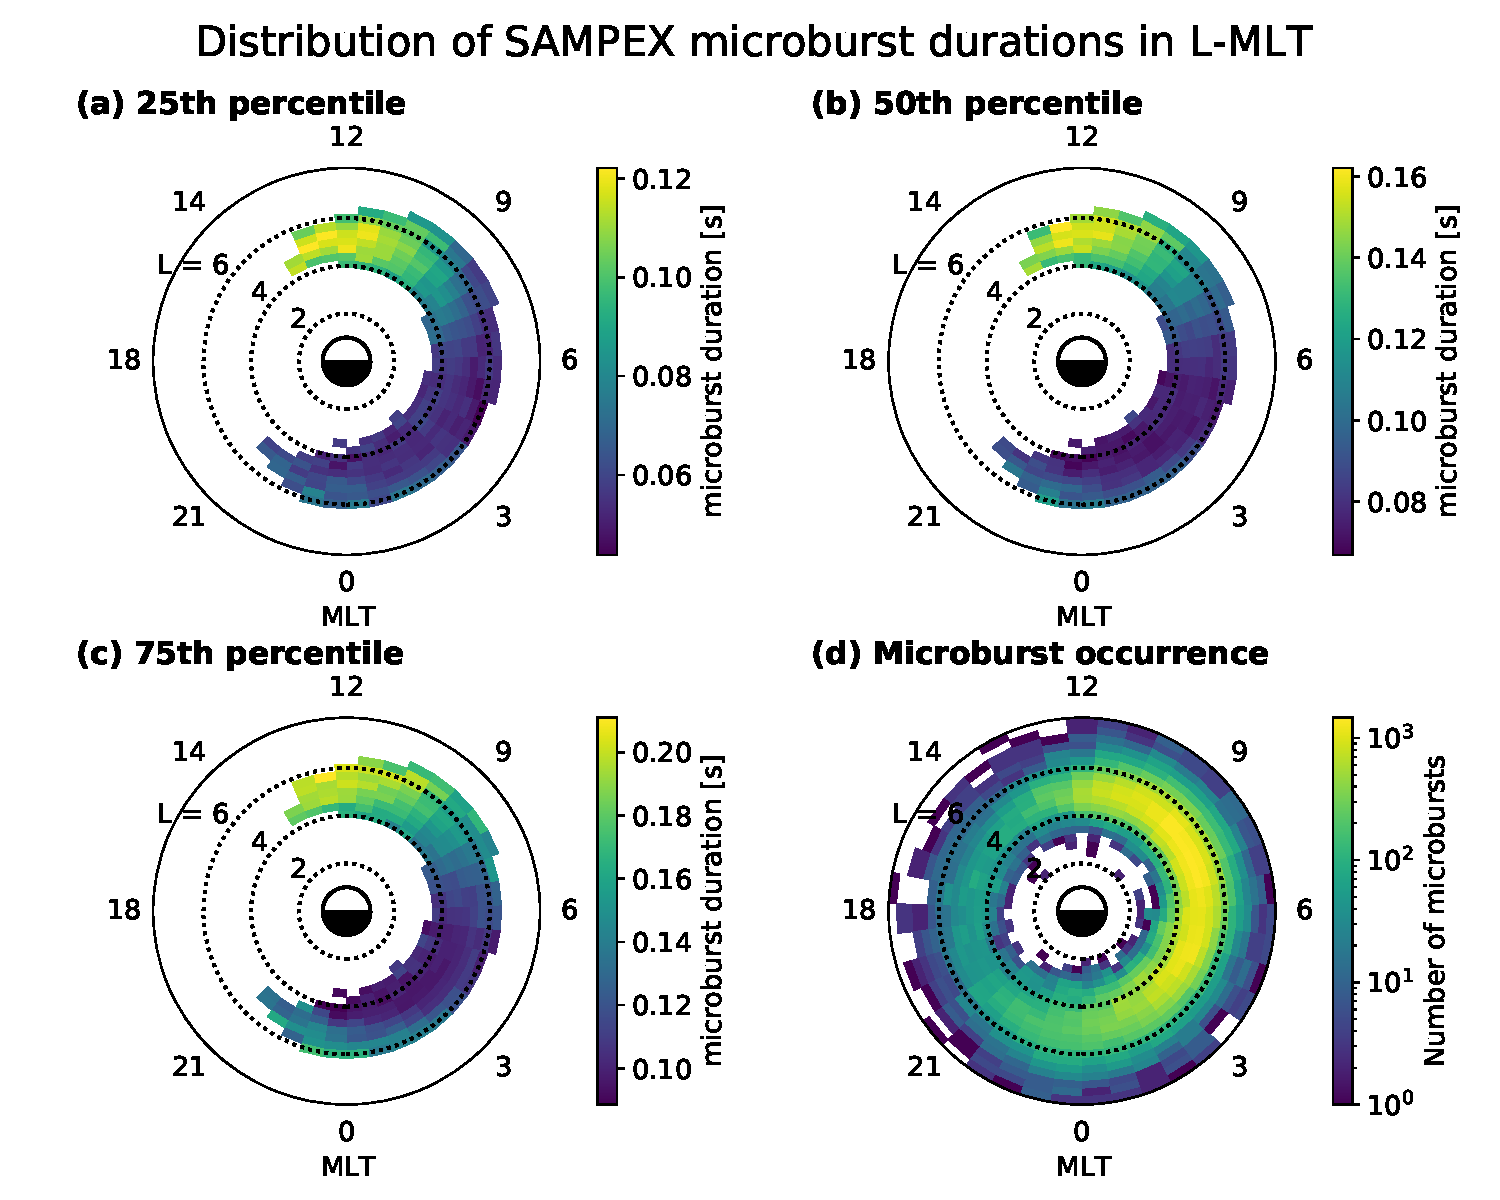
\includegraphics[width=\textwidth]{figures/fig3.pdf}
\caption{The joint distributions of microburst duration (FWHM) as a function of L and MLT. In each L-MLT bin with more than 100 good microburst fits, the 25th, 50th, and 75th percentiles of the duration were calculated and shown in panels a-c, respectively. The white bins in panels a-c have less than 100 good microburst fits. Panel d shows the distribution of the number of microbursts with 0 microbursts shown with the white bins.}
\label{fig3}
\end{figure}

\begin{figure}
\noindent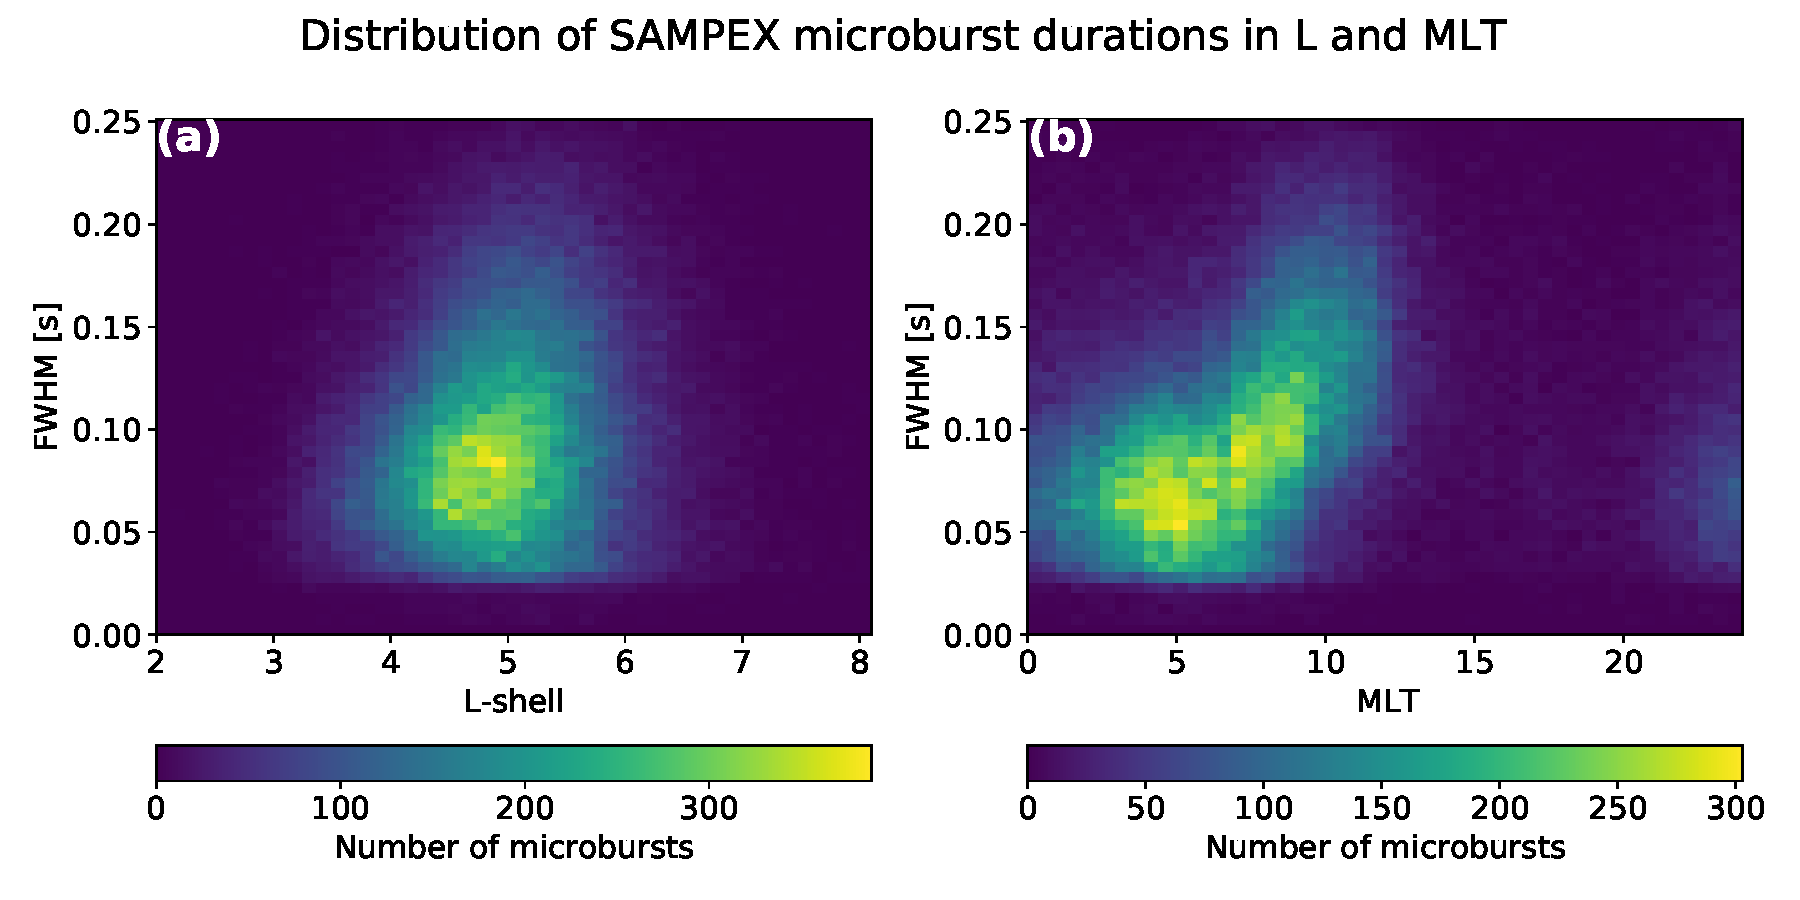
\includegraphics[width=\textwidth]{figures/fig4.pdf}
\caption{The marginalized distributions of the number of microbursts as a function of microburst duration (FWHM) and L shell in panel a and MLT in panel b.}
\label{fig4}
\end{figure}

\section{Discussion and Conclusions}\label{discussion}
We first addressed the possible burst parameter bias to narrower microbursts. We used the microburst identification algorithm with three background values: $A_{500}$, $A_{1000}$, and $A_{2000}$. As described in section \ref{microburst_id}, a wider centered running average, $A$, will be more sensitive to wider and less prominent microbursts. Therefore this bias manifests itself as a relative excess of longer duration microbursts for a wider $A$. We identified a minor bias. The difference in the median microburst duration, using the microburst lists generated using $A_{500}$ and $A_{2000}$, was 14 ms (corresponding to a 14\% relative difference). Considering this bias and Fig. \ref{fig2}a, we believe that the majority of $>1$ MeV microbursts have a true duration around 100 ms and the $A_{500}$ is adequate to identify these microbursts.

While the $\approx 100$ ms median microburst duration shown in Fig. \ref{fig2}a is in agreement with prior studies \cite<e.g.>{Anderson1964, Trefall1966, Nakamura2000}, we visually found a subtle and unexplored trend in the literature where the microburst duration is longer at lower energies \cite<e.g.>{Datta1997, Johnson2020, Shumko2020a}. This trend is consistent with recent modeling by \citeA{Chen2020} and \citeA{Miyoshi2020}, but it needs to be fully explored with energy-resolved measurements provided by, for example, FIREBIRD-II.

The microburst duration trend in L-shell is subtle; the 75th percentile of the duration distribution shown in in Fig. \ref{fig3}c near midnight slightly increases at higher L-shells. This is also noticeable in Fig. \ref{fig4}a. In contrast, the duration trend as a function of MLT is significant. The median microburst duration doubles from 80 to 160 ms between midnight and noon MLT. We now shift our focus to the MLT microburst duration trend.

Because chorus rising tone elements are believed to scatter microburst electrons \cite<e.g.>{Breneman2017, Saito2012, Miyoshi2020}, we will first review the observed chorus rising tone trends, and then compare it to our results.

Two recent studies by \citeA{Teng2017} and \citeA{Shue2019} quantified the properties of equatorial lower band (0.1-0.5 of the electro gyrofrequency) chorus rising tone elements. Both studies found that the rising tone element duration distribution peaks at $\approx 250$ ms around midnight MLT. Towards noon, this distribution broadens and the peak shifts to $\approx 500$ ms. Furthermore, \cite{Teng2017} found that the rising tone element duration distribution is broad and peaks at $\approx 500$ ms when $AE < 100$ nT and the distribution narrows and shifts to $\approx 250$ ms for $AE > 300$ nT. Both of these trends in MLT are similar to the microburst duration trends we found in Fig \ref{fig2}b and \ref{fig4}b, however the predictions point to a different wave property controlling the microburst duration.

Figure 4 in \citeA{Chen2020} shows a test particle model result and describe what wave properties bound the microburst duration in time-energy space. Medium energy (tens of keV to a few hundred keV) microburst duration is controlled by the rising tone element bandwidth. However, for higher energies the microburst duration is controlled by the wave's lower frequency and the upper magnetic latitude propagation. Different model parameters may change what wave properties are responsible for scattering $>1$ MeV microburst electrons, however \citeA{Shue2019} found that the rising tone element bandwidth is qualitatively the same between midnight and noon MLT. Between the chorus bandwidth and duration, the chorus rising tone element duration observations show a similar trend. Yet the theory does not conclusively predict what chorus wave properties control the $> 1$ MeV microburst duration. This question is left for future studies.

\textcolor{blue}{Check my arguments for clarity.} High latitude chorus waves, found at $\approx 10-25$ degrees magnetic latitude off of the equator, can also play at important role at scattering microburst electrons \cite{Lorentzen2001a}. \citeA{Li2009a} found that the majority of high latitude chorus waves are constrained to 6-12 MLT. Thus, it is tempting to conclude that the longer duration microbursts can be attributed to the low and high latitude chorus waves. However, because low latitude chorus waves are observed at 0-12 MLT \cite{Li2009a}, the resulting microburst duration distribution would reflect their superposition in the 6-12 MLT. If the two types of chorus waves scattered microbursts with different durations, Fig. \ref{fig4}b would show the durations broaden or bifurcate from midnight to noon MLT. Because Fig. \ref{fig4}b only shows the microburst duration shifting to longer durations, high vs low latitude chorus waves are an unlikely explanation for the microburst duration trend in MLT.

In summary, we found that the $>1$ MeV microburst duration distribution is peaked at 100 ms, with 75\% of microbursts narrower than 140 ms. We found no significant trend in the microburst duration as a function of L-shell, but we did find a strong trend as a function of MLT---the median microburst duration roughly doubles from 80 ms at midnight, to 160 ms at noon MLT. We found that the microburst duration trend in MLT to be similar to the trend in the rising tone element duration. However, contrary to the theoretically expected dependence of micriburst duration on chorus bandwidth, \citeA{Shue2019} did not find an incerase in the chorus rising tone bandwith between midnight and noon MLT.

%%%%%%%%%%%%%%%%%%%%%%%%%%%%%%%%
%% Optional Appendix goes here
%
% The \appendix command resets counters and redefines section heads
%
% After typing \appendix
%
%\section{Here Is Appendix Title}
% will show
% A: Here Is Appendix Title
%
%\appendix
%\section{Here is a sample appendix}

\acknowledgments
We are thankful for the engineers and scientists who made the SAMPEX mission possible. M. Shumko is thankful for the support provided by the NASA Postdoctoral Program at the NASA’s Goddard Space Flight Center, administered by Universities Space Research Association under contract with NASA. \textcolor{red}{Lauren's and Alex's funding sources} The SAMPEX HILT and attitude data are located at \url{http://www.srl.caltech.edu/sampex/DataCenter/data.html} and the minute cadence Auroral Electroject data is located at \url{ftp://ftp.ngdc.noaa.gov/STP/GEOMAGNETIC_DATA/INDICES/AURORAL_ELECTROJET/ONE_MINUTE/}.
The analysis software is archived at \textcolor{red}{\url{https://github.com/mshumko/sampex_microburst_widths}}.


%% ------------------------------------------------------------------------ %%
%% References and Citations

%%%%%%%%%%%%%%%%%%%%%%%%%%%%%%%%%%%%%%%%%%%%%%%
%
% \bibliography{<name of your .bib file>} don't specify the file extension
%
% don't specify bibliographystyle
%%%%%%%%%%%%%%%%%%%%%%%%%%%%%%%%%%%%%%%%%%%%%%%

\bibliography{refs.bib}



%Reference citation instructions and examples:
%
% Please use ONLY \cite and \citeA for reference citations.
% \cite for parenthetical references
% ...as shown in recent studies (Simpson et al., 2019)
% \citeA for in-text citations
% ...Simpson et al. (2019) have shown...
%
%
%...as shown by \citeA{jskilby}.
%...as shown by \citeA{lewin76}, \citeA{carson86}, \citeA{bartoldy02}, and \citeA{rinaldi03}.
%...has been shown \cite{jskilbye}.
%...has been shown \cite{lewin76,carson86,bartoldy02,rinaldi03}.
%... \cite <i.e.>[]{lewin76,carson86,bartoldy02,rinaldi03}.
%...has been shown by \cite <e.g.,>[and others]{lewin76}.
%
% apacite uses < > for prenotes and [ ] for postnotes
% DO NOT use other cite commands (e.g., \citet, \citep, \citeyear, \nocite, \citealp, etc.).
%



\end{document}



More Information and Advice:

%% ------------------------------------------------------------------------ %%
%
%  SECTION HEADS
%
%% ------------------------------------------------------------------------ %%

% Capitalize the first letter of each word (except for
% prepositions, conjunctions, and articles that are
% three or fewer letters).

% AGU follows standard outline style; therefore, there cannot be a section 1 without
% a section 2, or a section 2.3.1 without a section 2.3.2.
% Please make sure your section numbers are balanced.
% ---------------
% Level 1 head
%
% Use the \section{} command to identify level 1 heads;
% type the appropriate head wording between the curly
% brackets, as shown below.
%
%An example:
%\section{Level 1 Head: Introduction}
%
% ---------------
% Level 2 head
%
% Use the \subsection{} command to identify level 2 heads.
%An example:
%\subsection{Level 2 Head}
%
% ---------------
% Level 3 head
%
% Use the \subsubsection{} command to identify level 3 heads
%An example:
%\subsubsection{Level 3 Head}
%
%---------------
% Level 4 head
%
% Use the \subsubsubsection{} command to identify level 3 heads
% An example:
%\subsubsubsection{Level 4 Head} An example.
%
%% ------------------------------------------------------------------------ %%
%
%  IN-TEXT LISTS
%
%% ------------------------------------------------------------------------ %%
%
% Do not use bulleted lists; enumerated lists are okay.
% \begin{enumerate}
% \item
% \item
% \item
% \end{enumerate}
%
%% ------------------------------------------------------------------------ %%
%
%  EQUATIONS
%
%% ------------------------------------------------------------------------ %%

% Single-line equations are centered.
% Equation arrays will appear left-aligned.

Math coded inside display math mode \[ ...\]
 will not be numbered, e.g.,:
 \[ x^2=y^2 + z^2\]

 Math coded inside \begin{equation} and \end{equation} will
 be automatically numbered, e.g.,:
 \begin{equation}
 x^2=y^2 + z^2
 \end{equation}


% To create multiline equations, use the
% \begin{eqnarray} and \end{eqnarray} environment
% as demonstrated below.
\begin{eqnarray}
  x_{1} & = & (x - x_{0}) \cos \Theta \nonumber \\
        && + (y - y_{0}) \sin \Theta  \nonumber \\
  y_{1} & = & -(x - x_{0}) \sin \Theta \nonumber \\
        && + (y - y_{0}) \cos \Theta.
\end{eqnarray}

%If you don't want an equation number, use the star form:
%\begin{eqnarray*}...\end{eqnarray*}

% Break each line at a sign of operation
% (+, -, etc.) if possible, with the sign of operation
% on the new line.

% Indent second and subsequent lines to align with
% the first character following the equal sign on the
% first line.

% Use an \hspace{} command to insert horizontal space
% into your equation if necessary. Place an appropriate
% unit of measure between the curly braces, e.g.
% \hspace{1in}; you may have to experiment to achieve
% the correct amount of space.


%% ------------------------------------------------------------------------ %%
%
%  EQUATION NUMBERING: COUNTER
%
%% ------------------------------------------------------------------------ %%

% You may change equation numbering by resetting
% the equation counter or by explicitly numbering
% an equation.

% To explicitly number an equation, type \eqnum{}
% (with the desired number between the brackets)
% after the \begin{equation} or \begin{eqnarray}
% command.  The \eqnum{} command will affect only
% the equation it appears with; LaTeX will number
% any equations appearing later in the manuscript
% according to the equation counter.
%

% If you have a multiline equation that needs only
% one equation number, use a \nonumber command in
% front of the double backslashes (\\) as shown in
% the multiline equation above.

% If you are using line numbers, remember to surround
% equations with \begin{linenomath*}...\end{linenomath*}

%  To add line numbers to lines in equations:
%  \begin{linenomath*}
%  \begin{equation}
%  \end{equation}
%  \end{linenomath*}



